\chapter{Background}\label{chap:background}
This chapter offers an introduction to some key notions required to understand the rest of this document.
%
We start off by looking into formal languages and associated definitions in \autoref{sec:languages}, where we also define regular expressions and capturing groups, the main goals of our synthesis procedure\footnote{Definitions and examples in \autoref{sec:languages} were, in part, adapted from Chapter~3 of \textit{Compilers: Principles, Techniques, and Tools}, by \citet*{DragonBook} and Chapter~2 of \textit{Handbook of Formal Languages, Volume 1: Word, Language, Grammar}, by \citet{HandbookFormalLanguages1}}.
%
In \autoref{sec:logic} we introduce some well-known logic problems as well as the necessary definitions and notation\footnote{Definitions and examples in \autoref{sec:logic}
were, in part, adapted from \textit{Handbook of Satisfiability}, by \citet*{HandbookSAT} and Miguel Neves's MSc. Thesis: \textit{Distributed Solver for Maximum Satisfiability} \cite{MiguelThesis}}.
%
Finally, in \autoref{sec:back-ps}, we present an overview of the basic concepts of program synthesis.

\section{Regular Languages}\label{sec:languages}
Formal languages differ from the common meaning of the word \textit{language} in that they are built from a set of well-defined rules and thus stringently specified. Programming languages, such as \texttt{C} or \texttt{Python}, are examples of formal languages. They have a strict syntax and no deviation is tolerated: if a string does not comply with the syntax rules, it is not in the language.

To define a formal language, we must first define an alphabet.
An alphabet is a nonempty finite set whose elements are called the symbols, letters or tokens.
Symbols of the alphabet can be, for example, letters, digits, or punctuation marks. Alphabets are usually identified by capital Greek letters.

\begin{definition}[Alphabet]
An alphabet \(\Sigma\) is a nonempty finite set of symbols.
\end{definition}

\begin{example}
The following are examples of alphabets:

\begin{itemize}
\item \(\Sigma_1 = \{0,1\}\): the binary alphabet,
\item \(\Sigma_2 = \{a,b,c,d,e,f,g,h,i,j,k,l,m,n,o,p,q,r,s,t,u,v,w,x,y,z\}\): the Latin lowercase alphabet.
\end{itemize}
\end{example}

Typically, the alphabets used in programming applications are larger than \(\Sigma_1\) or \(\Sigma_2\).
The ASCII alphabet, for instance, contains 128 symbols which include all non-accentuated upper- and lower-case letters, digits, and most punctuation marks.
Unicode characters, which include 154 modern and historical scripts, as well as multiple symbol sets, are more inclusive, and are the most commonly used in practice. In its current version, Unicode 13.0, this alphabet contains close to 150 thousand characters\footnote{\url{https://www.unicode.org/charts}. Accessed on \formatdate{24}{10}{2020}}.

Given an alphabet, we can define strings (also called sentences or words) over it, which result from the concatenation of a finite number of the alphabet's symbols. Strings are usually identified by lower case letters and written between single quotes. The length of a string \(s\), denoted \(|s|\), is the number of symbols in it.

\begin{definition}[String]
A string \(s\) over an alphabet \(\Sigma\) is a finite sequence of symbols drawn from \(\Sigma\).
\end{definition}

\begin{definition}[Length of a string]
The length of a string \(s\), \(|s|\), is the number of symbols in \(s\).
\end{definition}

\begin{example}
The following are examples of strings:
\begin{itemize}
\item \(\epsilon\), the empty string, is the string of length zero,\par
\item \(s_1 = \) \textit{synthesis} is a string over alphabet \(\Sigma_2\) and it has length \(|s_1| = 9\).
\end{itemize}
\end{example}

At last, a language is a (finite or infinite) countable set of strings over some alphabet. Languages are usually identified by calligraphic capital letters.

\begin{definition}[Language]
A language \(\mathcal{L}\) is a countable set of strings over some fixed alphabet \(\Sigma\).
\end{definition}

\begin{example}
The following are examples of languages:
\begin{itemize}
\item \(\emptyset\), the empty set, is a language which contains no strings,\par
\item \{\(\epsilon\)\} is the language that contains only the empty string.
\end{itemize}
\end{example}

\subsection{Regular Operations}
Regular operations are a type of operation over languages, and regular languages are a subset of languages that are closed under regular operations. The three most basic regular operations are union, concatenation and closure.

The union of two languages \(\mathcal{L}\) and \(\mathcal{M}\), denoted \(\mathcal{L} \cup \mathcal{M}\), is the set of all strings in \(\mathcal{L}\) and all strings in \(\mathcal{M}\) (including those that are in both).
The concatenation of two languages \(\mathcal{L}\) and \(\mathcal{M}\), denoted \(\mathcal{L}\mathcal{M}\), is the set all strings formed by taking any string from \(\mathcal{L}\) and any string from \(\mathcal{M}\) and concatenating them. The concatenation of the same language, \(\mathcal{L}\), \(n\) times is sometimes denoted as \(\mathcal{L}^n\). For example  \(\mathcal{L}^3 = \mathcal{L}\mathcal{L}\mathcal{L}\).
The Kleene closure\footnotemark{} (also called Kleene star or simply star) of a language \(\mathcal{L}\), denoted \(\mathcal{L}^*\), is the set of strings resulting from the concatenation of any string in \(\mathcal{L}\) zero or more times. The Kleene closure of any language always includes the empty string.

\footnotetext{Kleene closure owes its name to the American mathematician Stephen Cole Kleene, who first described the concepts of regular language and regular expression in the~1950s.}
\begin{definition}[Regular operations] There are 3 regular operations on languages, union, concatenation and closure, which are defined as follows:
\begin{itemize}
\item Union: \(\mathcal{L} \cup \mathcal{M} = \{s :s \in \mathcal{L}\) \text{ or } \(s \in \mathcal{M}\}\),

\item Concatenation: \(\mathcal{L}\mathcal{M} =\{st : s \in \mathcal{L} \text{ and } t \in \mathcal{M}\}\),

\item Kleene closure: \(\mathcal{L}^*\) = \(\bigcup_{i=0}^\infty \mathcal{L}^i\).
\end{itemize}
\end{definition}

\subsection{Regular Expressions} \label{sec:back-regex}
Regular expressions (often shortened to \textit{regexes}) are used to describe regular languages. The language defined by a regular expression \(r\) is represented as \(\mathcal{L}(r)\).
Regular expressions are built recursively out of smaller regular expressions connected by operators. The simplest regular expressions refer to languages that contain just one symbol and are represented as that symbol in monospaced font.

\begin{example}
The regular expression \regex{a} defines the language \(\mathcal{L}({\regexm{a}}) =\) \{\textit{a}\}.
\end{example}{}

\begin{table}[t]
\centering

\newcolumntype{R}{>{\arraybackslash}m{.18\textwidth}}
\newcolumntype{L}{>{\arraybackslash}m{.2\textwidth}}
\newcolumntype{M}{>{\arraybackslash}m{.15\textwidth}}
\setlength\extrarowheight{.5em}

\begin{tabular}{l c c}
\toprule
Name & \makecell{Operation on\\regular expressions} & \makecell{Operation on\\languages} \\ \midrule
Union          & \(r|q\) & \quad \(\mathcal{L}(r) \cup \mathcal{L}(q)\) \\
Concatenation  & \(rq\)  & \quad \(\mathcal{L}(r)\mathcal{L}(q)\) \\
Kleene closure & \(r^*\) & \quad \(\mathcal{L}(r)^*\)\\
%  &  Positive closure of \(\mathcal{L}\)                  & \quad \(\mathcal{L}^*\) = \(\cup_{i=1}^\infty \mathcal{L}^i\)                                                           \\ 
\bottomrule
\end{tabular}
\caption{Regular operations}
\label{tab:regex-ops}
\end{table}


All regular operations have a counterpart operation on regular expressions. For example, the union of two regular expressions \(r\) and \(q\) results in a regular expression that defines the regular language \(\mathcal{L}(r) \cup \mathcal{L}(q)\). 
Since regular languages are closed under regular operations, it is possible to apply these operations to any regular expression.
The operations in regular expressions are generally represented in the same way as their regular-language counterparts, with the exception of union, which is represented using a \(|\) instead of the usual set notation~\(\cup\). The operations on regular expressions and their equivalent regular operations  are defined in \autoref{tab:regex-ops}.

The unary operator * has highest precedence, concatenation has second highest precedence and operator \(|\) has lowest precedence.
All three operators are left associative. Parentheses can be used to ensure a sub-expression takes precedence over the rest.

\begin{example}
\regex{a|b*c} is a regular expression that defines the language
\[\mathcal{L}(\regexm{a|b*c}) = \{a\} \cup \{b\}^* \{c\}\]
over the alphabet \(\Sigma = \{a, b, c\}\). This language contains strings that are either a single \(a\) or zero or more \(b\)s followed by one \(c\).
\end{example}

If two regular expressions \(r\) and \(s\) denote the same regular language, we say they are equivalent and write \(r = s\). For instance, \regex{a|b} = \regex{b|a}. % There are several algebraic laws that hold for arbitrary regular expressions, some of which are defined in \autoref{tab:regex-laws}.

% \begin{table}[t]
\centering
\begin{tabular}{@{}c c@{}}
\toprule
Algebraic Law                      & \quad Description                                    \\ \midrule
\(r|s = s|r\)                      & \quad Union is commutative                           \\
\(r|(s|t) = (r|s)|t\)              & \quad Union is associative                           \\
\(r(st) = (rs)t\)                  & \quad Concatenation is associative                   \\
\(r(s|t) = rs|rt; (s|t)r = sr|tr\) & \quad Concatenations distributes over union          \\ 
%\(\epsilon r = r\epsilon = r\)     & \quad \(\epsilon\) is the identity for concatenation \\ 
%\(r^* = (r|\epsilon)^*\)           & \quad \(\epsilon\) is guaranteed in a Kleene closure \\ 
\(r|r = r\)      & \quad Union is idempotent \\
\(r^{**} = r^*\)   & \quad * is idempotent \\
\(r?? = r?\)       & \quad ? is idempotent \\
\(r^{++} = r^+\)   & \quad + is idempotent \\

\(r^{+*} = r^{*+} = r^*\)  & \quad .......... \\
\(r?^* = r^*? = r^*\)      & \quad .......... \\
\(r?^+ = r^+? = r^*\)      & \quad .......... \\ \bottomrule
\end{tabular}
\caption{Algebraic laws for regular expression operators}
\label{tab:regex-laws}
\end{table}

\medskip
Since the introduction of regular expressions with the basic operators for union, concatenation, and Kleene closure, some new operators have been defined for regular expressions with the purpose of easing the specification of certain string patterns. Here we show some of those commonly used operators: \(+\), \(?\), \(\{m\}\), \(\{m,n\}\), and character classes.

The unary postfix operator \(+\) represents positive closure, which can be interpreted as `one or more occurrences of' (note the similarity to Kleene closure, `zero or more instances of'). It can be defined as
\[r^+ = rr^* = r^*r,\]
and gives rise to a new algebraic law:
\[r^* = r^+|\epsilon.\]
%
The unary postfix operator \(?\), often called \textit{option}, means `zero or one
occurrences of', and can be defined~as
\[ r? = r|\epsilon. \]
%
The range operators, \(\{m\}\) and \(\{m,n\}\), specify how many occurrences of the preceding regular expression they match. \(\{m\}\) is interpreted as `exactly \(m\) copies of', and \(\{m,n\}\) is interpreted as `at least \(m\) and at most \(n\) copies of'. For example:
\[r\{3\} = rrr,\]
\[r\{1,3\} = r|rr|rrr = rr?r?.\]
%
The operators \(+\), \(?\), \(\{m\}\) and \(\{m,n\}\) have the same precedence and associativity as operator~\(*\).


Character classes are a form of regular expression shorthand notation. A regular expression \(a_1|a_2|a_3|...|a_n\), where each \(a_i\) is a symbol of the alphabet, can be replaced by the shorthand \([a_1 a_2...a_n]\).
When \(a_1 a_2...a_n\) form a logical sequence, e.g., consecutive uppercase letters, lowercase letters, or digits, we
can replace them by \(a_1\mhyphen a_n\), that is, just the first and last tokens separated by
a hyphen.

%\mathchardef\mhyphen="2D

\begin{example}
The following are examples of character classes:
\begin{itemize}
\item \regex{[abc]} = \regex{a|b|c}
\item \regex{[a\mhyphen z]} = \regex{a|b|...|z}
\item \regex{[a\mhyphen z0\mhyphen 9]} = \regex{a|b|...|z|0|1|...|9}
\end{itemize}
\end{example}

\subsection{Capturing Groups}

Regular expressions can be coupled with capturing groups.
%
A capturing group is a sub-regex within a regex, usually specified with parentheses. %, which can be nested.
When a string is matched by a regular expression with capturing groups, the match operation returns the resulting captures, i.e., the text that is matched by the regex inside each pair of parentheses. Capturing groups are used to extract information from text. Once extracted, that information can be used independently from the original string.
Besides producing a capturing group, the parentheses also cause the expression inside them to take precedence over the remaining operators in the regular expression.
For instance, if a quantifier is placed after the parentheses, it applies to the regular expression inside as~a~whole.

\begin{example}\label{ex:capturing-groups}
Consider the regular expression \(r_1\) = \UseVerb{date2} and the string \(s\) = ``19/08/1996''. The regex \(r_1\) matches the string \(s\). Because \(r_1\) has no capturing groups, no captures are produced.
%
Consider now \(r_2\) = \verb`([0-9]{2})/([0-9]{2})/([0-9]{4})`. \(r_2\) also matches \(s\) (it has the same base regular expression as \(r_1\)) and it has 3 capturing groups. Thus, when matched to \(s\), \(r_2\) produces the captures ``19'', ``08'', and ``1996''.
%
%Finally, consider \(r_3\) = \verb`(([0-9]{2})/([0-9]{2}))/[0-9]{4}`. \(r_3\) also matches \(s\) and it has 3 capturing groups, two of which are nested inside the third one. When matched to \(s\), \(r_3\) produces the captures ``19/08'', ``19'', and ``08''.
\end{example}

\noindent
In the domain of form validations, we focus primarily on the capture of integer values in the input strings. We use the notation \(\$i, i \in \{0, 1, ...\}\), to refer to the integer value of the text captured by the \((i+1)\)\textsuperscript{th}~group.

\begin{example}
Recall the string \(s\) = ``19/08/1996'' and regex \(r_2\) = \verb`([0-9]{2})/([0-9]{2})/([0-9]{4})` from \autoref{ex:capturing-groups}. When matched to \(s\), \(r_2\) produces the captures ``19'', ``08'', and ``1996''. Thus, \(\$0 = 19\), \(\$1 = 8\), and \(\$2 = 1996\).
\end{example}

\section{Constraint Solving}\label{sec:logic}
Constraint solving techniques are used to solve problems where the space of solutions is restricted by logical constraints.
Throughout this document we make extensive use of \acf{SMT} and \acf{MaxSMT} to model problems in our synthesis domain.
%
The \ac{SMT} problem can be seen as a generalisation of the \ac{SAT} problem. Similarly, the \ac{MaxSMT} problem is defined as a generalisation of \ac{MaxSAT}. The next sections provide a brief introduction to each of these formalisms.

\subsection{Propositional Satisfiability}

In logic and computer science, \ac{SAT} is the problem of, given a Boolean formula, determining if there exists an assignment of its variables that satisfies it.
%
In addition to its theoretical importance, \ac{SAT} has many practical applications in the field of Computer Science. In 1971, \ac{SAT} was the first problem proven to be NP-Complete \cite{DBLP:conf/stoc/Cook71}. This means that numerous decision problems can be reduced to the \ac{SAT} problem, and subsequently solved using an off-the-shelf \ac{SAT} solver.

\begin{definition}[Literal]
A literal \(l\) is a Boolean variable (\(l = x\)) or its complement (\(l = \neg x\)).
\end{definition}

\begin{definition}[Clause]
A clause \(c\) is a disjunction of literals: \(c = l_1 \lor l_2 \lor ... \lor l_k\).
\end{definition}

\noindent
\ac{SAT} formulas are usually represented in the \acf{CNF}. 

\begin{definition}[\ac{CNF} Formula]
A formula \(\phi\) in \ac{CNF} is a conjunction of clauses: \(\phi = c_1 \land c_2 \land ... \land c_n\).
\end{definition}

\begin{example}\label{ex:CNF_formula}
Consider the variables \(X = \{x_1, x_2, x_3\}\). Then, \(\phi_1 = (x_1 \lor x_2) \land (\neg x_1 \lor x_3)\) is a \ac{CNF} formula over \(X\).
\end{example}

\begin{definition}[Assignment]
Given a formula \(\phi\), an assignment is a mapping \(\nu:~X\rightarrow\{\true,\false\}\), where \(X\) is the set of variables in \(\phi\).
\end{definition}

\noindent
Given an assignment \(\nu : X \rightarrow \{\true, \false\}\) and a variable \(x \in X\), the positive literal \(x\) is satisfied by \(\nu\) if and only if \(\nu(x) = \true\) and the negative literal \(\neg x\) is satisfied by \(\nu\) if and only if \(\nu(x) = \false\); a clause is satisfied by \(\nu\) if and only if at least one of its literals is satisfied by \(\nu\); a formula in CNF is satisfied by \(\nu\) if and only if all of its clauses are satisfied by \(\nu\).

\begin{definition}[Model]
Given a propositional formula  \(\phi\) and an assignment \(\nu\), \(\nu\) is a model of \(\phi\) if and only if \(\nu\) satisfies \(\phi\).
\end{definition}

\begin{example}
Recall the \ac{CNF} formula from \autoref{ex:CNF_formula}: \(\phi_1 = (x_1 \lor x_2) \land (\neg x_1 \lor x_3)\). The assignment \(\nu_1 = \{x_1 \mapsto \false, x_2 \mapsto \true, x_3 \mapsto \true\}\) is a possible model of \(\phi_1\).
\end{example}

\subsection{Maximum Satisfiability}
The problem of finding an assignment \(\nu\) to the variables of a CNF formula that satisfies the maximum number of clauses possible is known as \ac{MaxSAT}.
Unlike \ac{SAT}, which was a decision problem, \ac{MaxSAT} is an optimisation problem.
In computer science, many optimisation programs can be reduced into \ac{MaxSAT}. Moreover, \ac{MaxSAT} can be used used to get insights about the \textit{unsatisfiable} instances.
A \ac{SAT} solver tells us that we cannot satisfy all clauses. A \ac{MaxSAT} solver tells us how many can be satisfied at most.

\begin{example}\label{ex:MaxSAT}
Consider the \ac{CNF} formula \(\phi_2 = (x_1 \lor x_2) \land (x_1 \lor \neg x_2) \land \neg x_1\).
No assignment can satisfy all clauses in this formula. 
However, there can be assignments that satisfy two of the clauses in \(\phi_2\).
For example, \(\nu_2 = \{x_1 \mapsto \true, x_2 \mapsto \true\}\) satisfies all but the last clause in \(\phi_2\): it is a \ac{MaxSAT} model for \(\phi_2\).
\end{example}

\noindent
An important variation of the \ac{MaxSAT} problem, known as \textit{partial} \ac{MaxSAT}, divides its clauses into two types: hard clauses, \(\phi_H\), and soft clauses, \(\phi_S\).
Partial \ac{MaxSAT} is then the problem of finding an assignment \(\nu\) to the variables of a \ac{CNF} formula that satisfies all hard clauses and as many soft clauses as~possible.

\begin{definition}[Model]
Let \((\phi_H, \phi_S)\) be an instance of partial \ac{MaxSAT}. An assignment \(\nu\) is a model for \((\phi_H, \phi_S)\) if and only if \(\nu\) satisfies all clauses in \(\phi_H\) and the maximum number possible in \(\phi_S\).
\end{definition}

\begin{example}
Consider an instance of partial \ac{MaxSAT} \((\phi_{H}, \phi_{S})\), with the hard clause \(\phi_{H} = \neg x_1\) and soft clauses \(\phi_{S} = (x_1 \lor x_2) \land (\neg x_1 \lor x_2) \land \neg x_2\).
The assignment \(\nu_2 = \{x_1 \mapsto \false, x_2 \mapsto \true\}\) is a model for \((\phi_{H}, \phi_{S})\), because it satisfies all hard clauses and as many soft clauses as possible.
\end{example}



\subsection{Satisfiability Modulo Theories}

Oftentimes, it is advantageous to express the problem at hand using more expressive logics. In this thesis we make extensive use of an extension of \ac{SAT}: \acf{SMT}. \ac{SMT} is the problem of satisfiability of formulas with respect to some background theory \(\mathcal{T}\), which defines the interpretations of certain function symbols. This allows us to incorporate fragments of first-order logic in \ac{CNF} formulas.

\begin{definition}[\(\mathcal{T}\)-atom]
A \(\mathcal{T}\)-atom \(t\) is a ground atomic formula in \(\mathcal{T}\).
\end{definition}


\begin{definition}[\(\mathcal{T}\)-literal]
A \(\mathcal{T}\)-literal is a \(\mathcal{T}\)-atom (\(t\)) or its negation (\(\neg t\)).
\end{definition}

\begin{definition}[\(\mathcal{T}\)-formula]
A \(\mathcal{T}\)-formula is then analogous to a propositional formula but it is composed of \(\mathcal{T}\)-literals instead of propositional literals.
\end{definition}

\noindent
The values in an \ac{SMT} assignment depend on the background theory~\(\mathcal{T}\). Commonly used theories include the theory of \ac{LIA}, whose values are integer, the theory of \textit{strings}, whose values are strings, and the theory of \ac{EUF}, which assigns functions with a valid interpretation. Given an \ac{SMT} assignment, \(\nu\), and a \(\mathcal{T}\)-atom \(t\), the positive \(\mathcal{T}\)-literal \(t\) is satisfied by \(\nu\) if and only if \(\nu(t)\) is assigned \true according to theory \(\mathcal{T}\) and the negative \(\mathcal{T}\)-literal \(\neg t\) is satisfied by \(\nu\) if and only if \(\nu(t)\) is assigned \false according to \(\mathcal{T}\); a \(\mathcal{T}\)-formula is satisfied by \(\nu\) if and only if all of its clauses are satisfied by \(\nu\).

\ac{SMT} is then the problem of deciding, given an SMT formula \(\phi\), if there exists an assignment of the variables and functions of \(\phi\) that satisfies it.

\begin{example}
Let \(\phi_3 = (b - a = 1) \land ((b<5) \lor (a>10))\) be a \ac{SMT} formula in the theory of LIA. A possible model for \(\phi_3\) is \(\nu_3 = \{a \mapsto 1, b \mapsto 2\}\).
\end{example}


\subsection{\acl{MaxSMT}}

The same way \ac{MaxSAT} finds the maximum number of clauses that can be satisfied in a \ac{CNF} formula, \ac{MaxSMT} finds the maximum number of clauses that can be satisfied in an unsatisfiable \(\mathcal{T}\)-formula.
We can also define \textit{partial} \ac{MaxSMT} with hard clauses, \(\phi_H\), and soft clauses, \(\phi_S\).

\begin{example}
Let \((\phi_{H}, \phi_{S})\) be a partial \ac{MaxSMT} instance, with hard clauses \(\phi_{H}=(b-a=1) \land (b<10)\) and soft clauses \(\phi_{S} = (b<5) \land (a>10)\). We can satisfy at most one of the soft clauses. Therefore \(\nu_3 = \{a \mapsto 1, b \mapsto 2\}\) is an optimal model for this instance.
\end{example}

\section{Program Synthesis} \label{sec:back-ps}
\begin{figure}
    \centering
    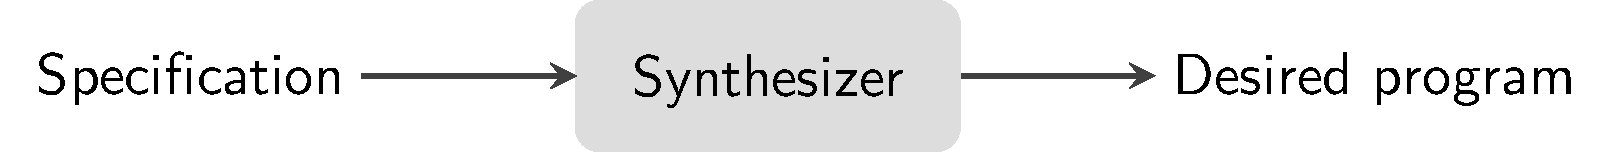
\includegraphics[scale=.35]{pictures/program_synthesis.pdf}
    \caption{Program Synthesis}
    \label{fig:program-synthesis}
\end{figure}

Program synthesis is the task of automatically generating a program that satisfies some desired behaviour expressed as a high-level specification~(see \autoref{fig:program-synthesis}).
This specification can range from a complete formal definition, such as a first-order formula \cite{DBLP:conf/ijcai/Green69,DBLP:conf/pldi/GulwaniJTV11}, to more ambiguous descriptions of the desired program's behaviour, like a set of input-output examples~\cite{DBLP:conf/iclr/BalogGBNT17,DBLP:conf/pldi/FengMBD18,DBLP:conf/icse/JhaGST10,DBLP:conf/ijcai/ShawWG75,DBLP:journals/jacm/Summers77,DBLP:conf/aaai/ManshadiGA13,DBLP:conf/ijcai/RazaGM15,DBLP:conf/aaai/MortonHSPS20} or a natural language sentence~\cite{DBLP:conf/icse/DesaiGHJKMRR16,DBLP:journals/pacmpl/Yaghmazadeh0DD17,DBLP:conf/naacl/HuangWSYH18,Regel20,DBLP:conf/aaai/ManshadiGA13,DBLP:conf/ijcai/RazaGM15}.

According to \citeauthor{PSnow}~\cite{DBLP:conf/ppdp/Gulwani10,PSnow}, a program synthesizer is typically characterised by three key dimensions:
\begin{enumerate*}[label=(\roman*)]
  \item the way the user specifies the desired characteristics of the program,
  \item the space of all possible programs the synthesizer can generate, and
  \item the search technique used to explore that~space.
\end{enumerate*}

\paragraph{Desired behaviour specification} is the most important characteristic of a synthesizer from the users' point of view.
It is the language in which they describe the behaviour of the program they intend to generate. 
It must take into consideration the underlying task, the users' technical background and which material is available when using the synthesizer.

\paragraph{Program space} is the set of all programs the synthesizer can possibly generate. In other words, it is the space over which the synthesizer searches for a feasible program. It depends on the domain of the problem the synthesizer is intended to solve. It must be expressive enough to ensure the desired program is included, but also restricted enough lest the search problem become intractable.

\paragraph{Search technique} refers to the method employed to find the desired program within the program space. It can be based on enumerative search, deductive search, constraint solving, or some combination thereof.

\medskip

\noindent
The three dimensions are further described in sections~\ref{sec:desired-behaviour-spec}, \ref{sec:program-space} and \ref{sec:search-technique}, respectively.

\subsection{Desired Behaviour Specification} \label{sec:desired-behaviour-spec}
For the synthesis procedure to start, the user must first specify the program's intended behaviour. The desired behaviour can be described in many different ways, and is internally converted to some sort of behavioural constraints, which the output program must satisfy.

\begin{definition}[Desired Behaviour Specification]
The desired behaviour specification is a predicate~\(\phi\), such that \(\phi(\vec{x}, y)\) is \true{} if and only if \(y\) is the desired output value for the input vector \(\vec{x}\).
\end{definition}

\noindent
The first approaches to automating the creation of programs, proposed in \citeyear{DBLP:conf/ijcai/Green69} \cite{DBLP:conf/ijcai/Green69,DBLP:conf/ijcai/WaldingerL69}, were based in deductive synthesis.
Such synthesizers work based on a complete formal specification of the desired program's behaviour.
Then, they employ a theorem prover to construct a proof of the provided specification from which it is able to extract the executable program~\cite{DBLP:conf/ijcai/Green69,DBLP:journals/cacm/MannaW71,DBLP:journals/toplas/MannaW80,DBLP:conf/ijcai/WaldingerL69}.

Deductive synthesizers require the user to provide a complete formal description of the desired behaviour, such as a first-order formula.
Because it is a complete definition, the synthesizer always returns a program with the exact desired behaviour, and it is always satisfactory to the user.
However, writing these kind of specifications can be as complex as writing the program itself, and might force the user to learn a new formalism in any case.

\begin{figure}
    \centering
    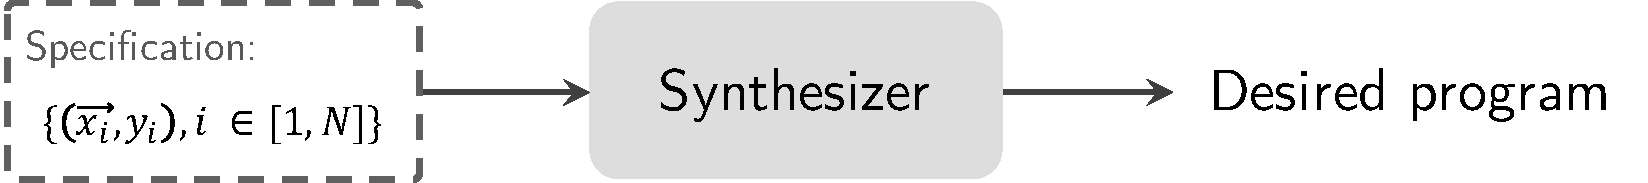
\includegraphics[scale=.35]{pictures/pbe.pdf}
    \caption{\ac{PBE}: The desired behaviour specification is a set of \(N\) input-output examples.}
    \label{fig:pbe}
\end{figure}

Such difficulties motivated a new approach to program synthesis: inductive synthesis \cite{DBLP:conf/pldi/FengMBD18,DBLP:conf/pldi/FengMGDC17,DBLP:conf/ijcai/ShawWG75,DBLP:journals/jacm/Summers77,UnchartIt20,Orvalho19,DBLP:journals/pvldb/OrvalhoTVMM20,AlphaRegex16,DanielThesis,PedroThesis}. The program is then built based on simpler (albeit ambiguous) specifications, easier for the user to devise. \acf{PBE} is a branch of inductive synthesis where the user intent is specified using input-output examples~\cite{DBLP:conf/pldi/GodefroidT12,DBLP:conf/ijcai/ShawWG75,DBLP:journals/jacm/Summers77,DBLP:conf/sigmod/WangCB17,DBLP:conf/pldi/WangCB17,DBLP:conf/pldi/FeserCD15,DBLP:conf/aaai/MortonHSPS20}, as shown in \autoref{fig:pbe}.
%\textcolor{red}{(\cite{DBLP:conf/ijcai/ShawWG75} synthesises simple LISP programs from one input-output example.~\cite{DBLP:journals/jacm/Summers77} from several output examples)} or natural language descriptions~\cite{DBLP:conf/icse/DesaiGHJKMRR16}).

\begin{definition}[Input-Output Examples]
Input-output examples are a type of incomplete specification defined as a set of \(N\) tuples:  \(\mathcal{X} = \{(\vec{x_i}, y_i), i \in \{1, ..., N\}\}\) where each \(y_i\) is the desired return value for input \(\vec{x_i}\).
\end{definition}

\begin{definition}[\acl{PBE}]
Programming by example is the problem of synthesising a program using input-output examples as a specification of the desired program behaviour. In programming by example, the behavioural constraint is
\[\bigwedge_{(x_i, y_i) \in \mathcal{X}} P(x_i) = y_i,\]
which states that program \(P\) is correct if it yields the correct output for the inputs specified in the specification.
%\[\phi(\vec{x}, y) = \neg (\exists z : (\vec{x}, z) \in \{(\vec{x_i}, y_i), i \in \{1, ..., N\}\} \wedge z \neq y)\]
\end{definition}

\begin{comment}
\begin{example}
Suppose we would like to generate a function which, for any integer input numbers \(x_1\) and \(x_2\) returns their sum:
\[f(x_1, x_2) = x_1 + x_2\]
A \ac{PBE} synthesiser would require some input-output examples as input, for example:
\[\{((1, 1), 2), ((1, 0), 1), ((2, 1), 3), ((2, 0), 2), ((1, 2), 3)\}\]
\end{example}
\end{comment}

\noindent
Input-output examples, although easier for the users to obtain and comprehend, are an incomplete specification. In general, there are several programs consistent with the provided specification even though not all of those correspond to the desired program and might not exhibit the behaviour expected by the user for cases that are not covered by the specification.

The ambiguity of input-output examples raises the necessity of selecting one among multiple candidate programs. One way to do this selection is by ranking the correct programs according to the measure of some characteristic that is desirable in programs of the domain in question, and returning to the user the program that ranks the highest~\cite{UnchartIt20,Regel20,DBLP:conf/ijcai/EllisG17,DBLP:conf/pldi/GveroKKP13,DBLP:conf/oopsla/PolozovG15,DBLP:conf/cav/SinghG15}.
Common desirable characteristics used to rank the programs include: execution speed (when we are looking for an efficient program), robustness (how well it generalises to new input-output examples), and readability (favours common operations in the underlying language, making it easy for the user to understand).
Another approach is to enable the synthesizer to interact with the user to try and disambiguate the underlying intent~\cite{DBLP:conf/sigmod/GulwaniM14,UnchartIt20,DBLP:journals/pvldb/LiCM15,DBLP:conf/sigmod/WangCB17,DBLP:conf/pldi/WangCB17,DBLP:conf/uist/MayerSGLMPSZG15}. Section~\ref{sec:rel-user-interaction} provides more details on this topic.

\subsection{Program Space} \label{sec:program-space}
The next step towards finding a program that satisfies the user's needs is defining the space of programs over which the synthesizer performs the search: the program space.
We cannot consider all the programs that can be written using a full-featured programming language. Too many programs would be taken into consideration, rendering the search space intractable.
On that account, we need to restrict the language in which the programs are written in order to enable an efficient search of the program space.
However, we must ensure it remains expressive enough to capture many real-world tasks within the considered specialised domain.
We call this language \acf{DSL}.
The choice of a synthesizer's \ac{DSL} is crucial: it must allow a good balance between expressiveness and efficiency.

\begin{definition}[\acl{DSL}]
Domain specific language is the restricted language in which the synthesised programs are written. It includes information about both form (syntax) and meaning (semantics).
\end{definition}

\noindent
We may impose restrictions on the allowed datatypes, as well as the operations over them so as to include only those relevant for the considered domain. For example, one could allow only integers and comparison operations, or arithmetic operations, or even only operations supported in some API exported by a given library. We can also restrict the program space by imposing constraints over the control structure of the program: we may disallow looping structures in the program, or bound the number of statements.

The constraints imposed on the language are named structural constraints, and they define the search space the synthesiser must consider. A \ac{CFG} is typically used to define the syntax of the \ac{DSL}.

\begin{definition}[Context-Free Grammar%
\footnote{Adapted from Chapter~2 of \textit{Speech and Language Processing} by \citet{Jurafsky}.}]
A \ac{CFG} is defined by a 4-tuple \((N, \Sigma, R, S)\), where:
\begin{itemize}[itemsep=.3ex]
    \item \(N\) is a set of non-terminal symbols,
    
    \item \(\Sigma\) is a set of terminal symbols (disjoint from \(N\)),
    
    \item \(R\) is a set of rules or productions, each of the form \(A \to \beta\), where:
    \begin{itemize}
        \item \(A\) is a non-terminal,
        \item \(\beta\) is a string of symbols from the infinite set of strings \((\Sigma \cup N)*\), and
    \end{itemize}
    
    \item \(S\) is a designated start symbol and a member of \(N\).

\end{itemize}
\end{definition}

\noindent
Then, a program on a \ac{DSL} is a production of the corresponding \ac{CFG} containing only terminal symbols, which include all operators and literal values in the \ac{DSL}.

Syntax-guided synthesis \cite{DBLP:conf/fmcad/AlurBJMRSSSTU13,DBLP:conf/aaai/MortonHSPS20} is the branch of program synthesis in which the user to supplies the language syntax (in the form of a grammar) alongside the behaviour specification. This provides structure to the program space, which may allow for a more efficient search method. Furthermore, the generated programs are more interpretable to the user and better adapted to the domain at hand, since they are derived from the given grammar. On the other hand, syntax-guided synthesis requires the user to have a deeper technical knowledge not only on the specific domain on which he or she is working but also on formal languages and how to define them.

%Restricted DSLs can also enable more efficient special-purpose search algorithms. For example, if we consider a DSL that allows only the concatenation of substrings of an input string, a dynamic programming can be used to efficiently enumerate all possible outputs and thus search on such a space~\cite{DBLP:conf/oopsla/PolozovG15}.

% string programming/expression language that supports restricted forms of regular expressions, conditionals and loops. Expressive SQL queries

\subsection{Search Technique}\label{sec:search-technique}

Program synthesis can be seen as a search problem. It aims at finding a program in the search space defined by structural constraints that satisfies the behavioural constraints.

\begin{definition}[Program Synthesis]
Given a specification of desired behaviour \(\phi\), program synthesis is the problem of finding a program \(P\) that satisfies~\(\phi\).
\end{definition}

\noindent
Several search techniques have been explored to solve program synthesis. In the remainder of this section, some of these search techniques are briefly explained. Note that one synthesizer does not have to apply only one of these techniques; more often, a combination of several techniques is applied.

\begin{figure}
    \centering
    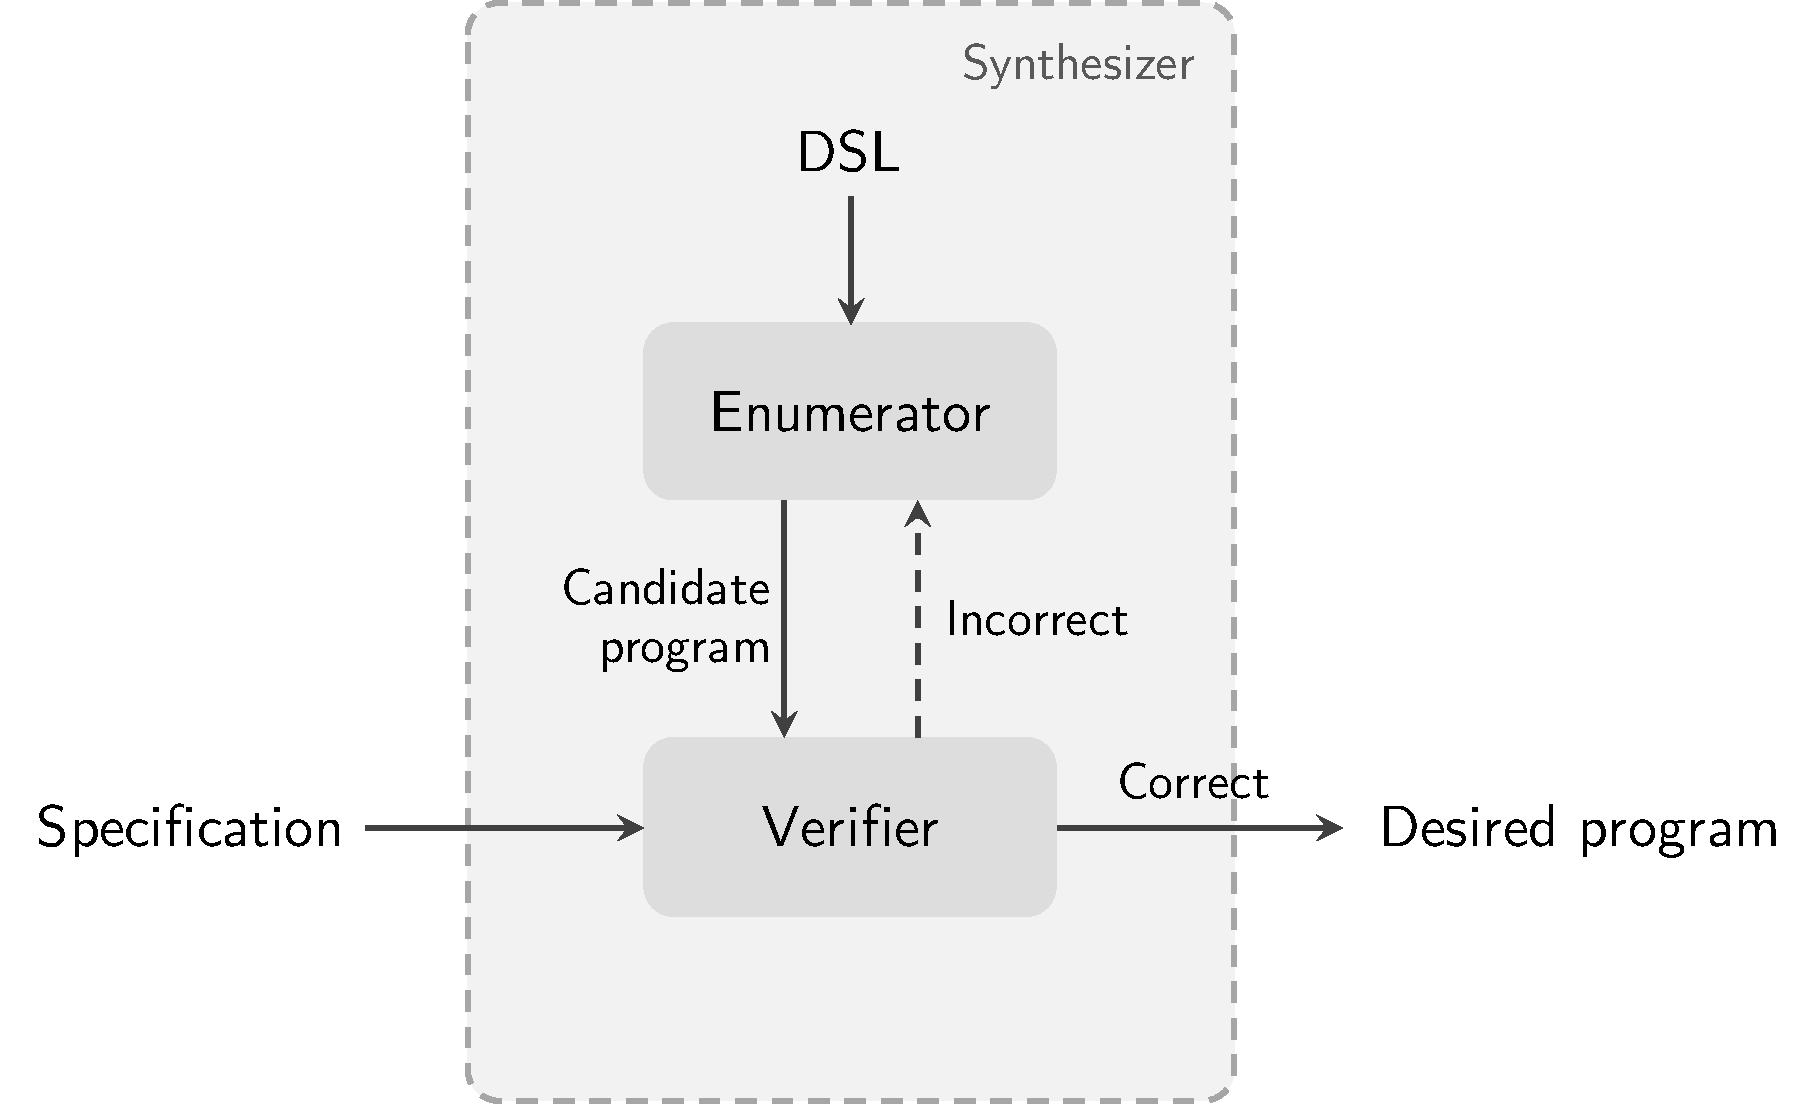
\includegraphics[scale=.35]{pictures/enumerative_search.pdf}
    \caption{Enumerative search}
    \label{fig:enumerative_search}
\end{figure}

\paragraph{Enumerative Search}\label{sec:enum-search}
\cite{DBLP:conf/pldi/FengMGDC17,DBLP:conf/pldi/FengMBD18,AlphaRegex16,Orvalho19,DBLP:conf/cav/ReynoldsBNBT19,DBLP:journals/pvldb/OrvalhoTVMM20} is a common approach to solve the search problem of program synthesis. In this technique, out synthesizer must include two key components: an \textit{enumerator} and a \textit{verifier}.
The \textit{enumerator} successively enumerates programs from the program space in some order. For each candidate program, the \textit{verifier} subsequently checks whether it satisfies all behavioural constraints, i.e., it is consistent with the user intent specification.
If the \textit{verifier} deems the program consistent with the given specification, then the program is correct and it can be returned to the user.
If, on the other hand, the \textit{verifier} decides that the given program does not satisfy the specification, then the \textit{enumerator} must pick a new program from the search space.
This loop is described in \autoref{fig:enumerative_search}.

A naive implementation of enumerative search does not scale to complex programs; however, it is a very effective strategy when coupled with some optimisation techniques. First off, the program space must be structured according to some metrics, usually program size or complexity, such that the \textit{enumerator} yields simpler programs first and only when those are refuted by the \textit{verifier} are more complex programs considered. This concept contributes to solving the problem of user intent ambiguity introduced in \autoref{sec:desired-behaviour-spec} by applying the Ockham's Razor principle: choose the simplest program that is consistent with the specification.

Another way to speed up enumerative search is by employing pruning techniques, such as discarding equivalent programs from the search space.
%The \textit{verifier} may also try to formulate a hint as to why a program deemed incorrect is not consistent with the specification and notify the \textit{enumerator}
In addition, when the \textit{verifier} rejects a program, it may apprise the \textit{enumerator} of the reason behind the program's incorrectness, thus reducing the program space and preventing the \textit{enumerator} from generating programs that fail in the same way.
This idea is further discussed in \autoref{sec:cegis}.

\paragraph{Deductive Search} \cite{DBLP:conf/oopsla/PolozovG15,DBLP:conf/ijcai/MannaW79,DBLP:conf/cav/ChenWBDF20} is based on a top-down propagation of constraints through the grammar that defines the program space. It recursively reduces the problem of synthesising an expression that satisfies a certain specification to simpler sub-problems, thereupon combining those results.

Suppose we want to synthesise an expression \(e\) of the form \(F(e_1, e_2)\) that complies with a specification \(\phi\). Deductive search would leverage the inverse semantics of \(F\) to push constraints on \(e\) down through the grammar into constraints on \(e_1\) and \(e_2\). Finding \(e_1\) and \(e_2\) are then simpler sub-problems whose solutions, once found, can be combined to produce the originally desired expression \(e\).

Deductive search is very convenient when the underlying grammar allows for a rich set of constants. In such cases, enumerative search is no longer viable: an enumeration step is required for each possible constant in order to find the right one, resulting in too many iterations. On the other hand, the top-down deductive technique can deduce constants based on the accumulated constraints as the last  step in the search process.

\paragraph{Constraint Solving} \cite{Solar-LezamaPhDThesis,DBLP:conf/popl/SrivastavaGF10} consists on somehow generating a logical formula whose solution yields the intended program, and then solving it.

Several approaches can be used to generate the formula. On one extreme, we have invariant-based methods, which generate one formula that is satisfiable if and only if the program is consistent with the specification. Upon solving such a formula, we have not only a correct program but also a inductive proof of its correctness.
However, these methods do not scale well with the complexity of the specification --- the resulting formula may be intractable, and much more complex than the program itself.
%
To circumvent this drawback, we can instead make use of input-based methods. Then, the formula asserts the correctness of the program only on a subset of all possible inputs, which leads to simpler constraints.

Once we have a logic formula, it must be solved. These formulas are of second-order logic, and need to be first reduced to first-order quantifier-free constraints that can the be solved using an off-the-shelf logic-based solver. Second-order reduction can be achieved using techniques such as \ac{CEGIS} \cite{Solar-LezamaPhDThesis,DBLP:conf/tacas/AhmedPA20}, which is described in \autoref{sec:cegis}.

